\section{Arquitectura del Sistema}

\subsection{Aquitectura de conexión}


\begin{figure}[!h]
	\centering
	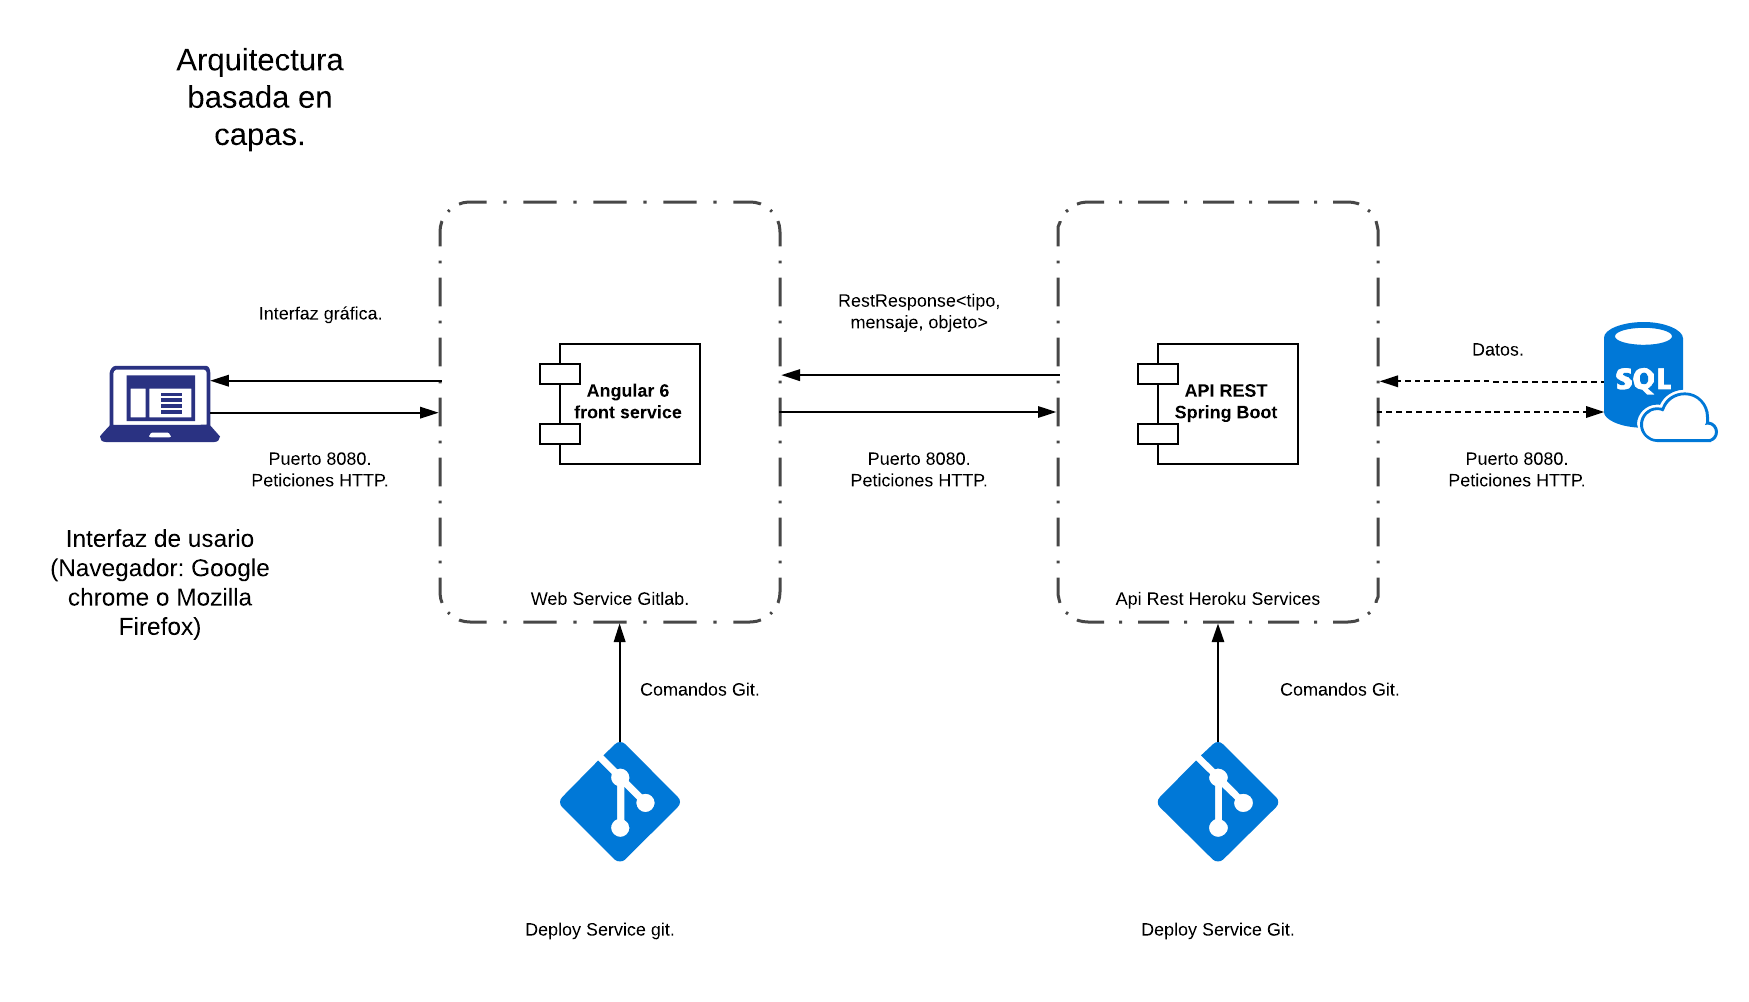
\includegraphics[width=0.8\linewidth]{images/Arquitectura/Blank_Diagram2.png}
	\caption{Representación gráfica de la conexión de servicios de la arquitectura del sistema.}
\end{figure}


La arquitectura del sistema propuesta es una arquitectura en capas, las cuales están definidas dentro de la figura 1. Está compuesta por:

\begin{itemize}
	\item Una capa de presentación (funcionalidad relacionada con la interfaz de usuario), una capa de negocios (procesamiento de reglas de negocios) y una capa de datos (funcionalidad relacionada con el acceso a datos).

	\item La capa de interfaz utiliza el framework angular para la interpretación  de los eventos ocurridos en el navegador por parte del usuario, el sistema está guardado en un servidor que provee gitlab basado en node js.

	\item La lógica del negocio se encuentra en un servidor que se encuentra alojado en los servidores de Heroku y está programado en java con el framework spring boot. Para la base de datos se utilizó una basada en relaciones, ésta está alojada en Amazon web Service.
\end{itemize}


\subsection{Lista de peticiones}

Por convención, se utilizará las peticiones propias del protocolo HTTP: GET, POST, PUT, DELETE.

\subsection{Formas de recibir información}

La información se enviara a través de paquetes JSON.

Por parte del servidor tenemos que se enviará la información con la siguiente forma:

\begin{figure}[!h]
    \centering
    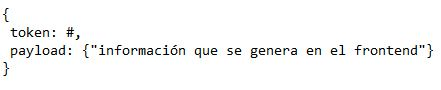
\includegraphics[width=0.7\linewidth]{images/Arquitectura/Captura.JPG}
    \caption{Representación gráfica de la estructura por petición del frontend al backend}
\end{figure}


A continuación se definen los campos de la Figura 2:
\begin{itemize}
    \item token: Este campo hace referencia a la información necesaria del usuario que hace la petición \newline al servidor del backend.
    \item payload: Este campo hace referencia a la información principal de que será procesada por\newline el servidor del backend.
\end{itemize}


Por parte del back al frontend tenemos que la información se enviará con la siguiente estructura:

\begin{figure}[!h]
    \centering
    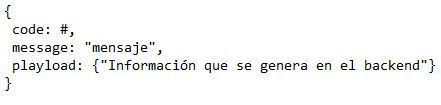
\includegraphics[width=0.7\linewidth]{images/Arquitectura/back.JPG}
    \caption{Representación gráfica de la estructura por petición del backend al frontend}
\end{figure}

A continuación se definen los campos de la Figura 3:
\begin{itemize}
    \item code: Este campo es un número que el servidor del backend enviará para verificar si la información se procesó correctamente o hubo un error.
    \item message: Este campo es un mensaje que el servidor del backend enviará para verificar si la información se procesó correctamente o hubo un error.
    \item payload: Este campo hace referencia a la información principal que fue recuperada de la base de datos y que será procesada por el servidor del frontend.
\end{itemize}

